\documentclass[solution, letterpaper]{cs20inclass}
\usepackage{enumerate}
\usepackage{tikz}
\usepackage{pgf}
\usepackage{tikz}
\usepackage{hyperref}
\begin{document}
\header{18}{Wednesday, March 9, 2016}

\noindent Author: Michelle Danoff, Tom Silver% \\

\paragraph*{Executive Summary}
\begin{enumerate}
\item Properties of binary relations
\begin{itemize}
\item \textit{Transitive}: A binary relation $R$ on the set $A$ is transitive iff\\$u R v \wedge v R w \implies u R w$ for all $u,v,w \in A$.
\item \textit{Reflexive}: $u R u$ for all $u \in A$.
\item \textit{Irreflexive}: $\neg(uRu)$ for all $u \in A$
\item \textit{Symmetric}: $u R w \implies w R u$ for all $u,w \in A$.
\item \textit{Antisymmetric}: $((u \neq w) \land (u R w)) \implies \neg(wRu)$ for all $u, w \in A$.
\item \textit{Asymmetric}: $u R w \implies \neg(wRu)$ for all $u, w \in A$.
\end{itemize}
\item Recall that $G$ is a binary relation on $V$, where $uGw$ means that there is an edge from $u$ to $w$.
\begin{itemize}
\item $G^+$ is transitive and is the \textit{transitive closure} of $G$. This means that $G^+$ is the minimal transitive relation that includes $G$ (i.e. $G \subseteq G^+$).
\item $G^*$ is reflexive, transitive, and the \textit{reflexive transitive closure} of $G$.
\end{itemize}
\item The vertices $u,v \in V$ are \textit{strongly connected} iff $uG^*v \wedge vG^*u$. That is, if there exists a walk from $u$ to $v$ and a walk back from $v$ to $u$.
\item Special types of relations
\begin{itemize}
\item \textit{Strict partial orders}: transitive and irreflexive
\item \textit{Weak partial orders}: transitive, reflexive, and antisymmetric
\item \textit{Equivalence relations}: transitive, reflexive, and symmetric
\item A relation $R$ is a weak partial order iff $R = D^*$ for some DAG $D$
\item A relation $R$ is a equivalence relation iff $R$ is the strongly connected relation of some digraph
\end{itemize}
\item An equivalence relation $R$ decomposes the domain into subsets called \textit{equivalence classes}, where $aRb$ iff $a$ and $b$ are in the same equivalence class.
\end{enumerate}

\problem
Draw one directed graph with 3 vertices $A, B, C$ for each of the following relationships
\subproblem Reflexive
\subproblem Symmetric
\subproblem Asymmetric
\subproblem Transitive


\begin{solution}
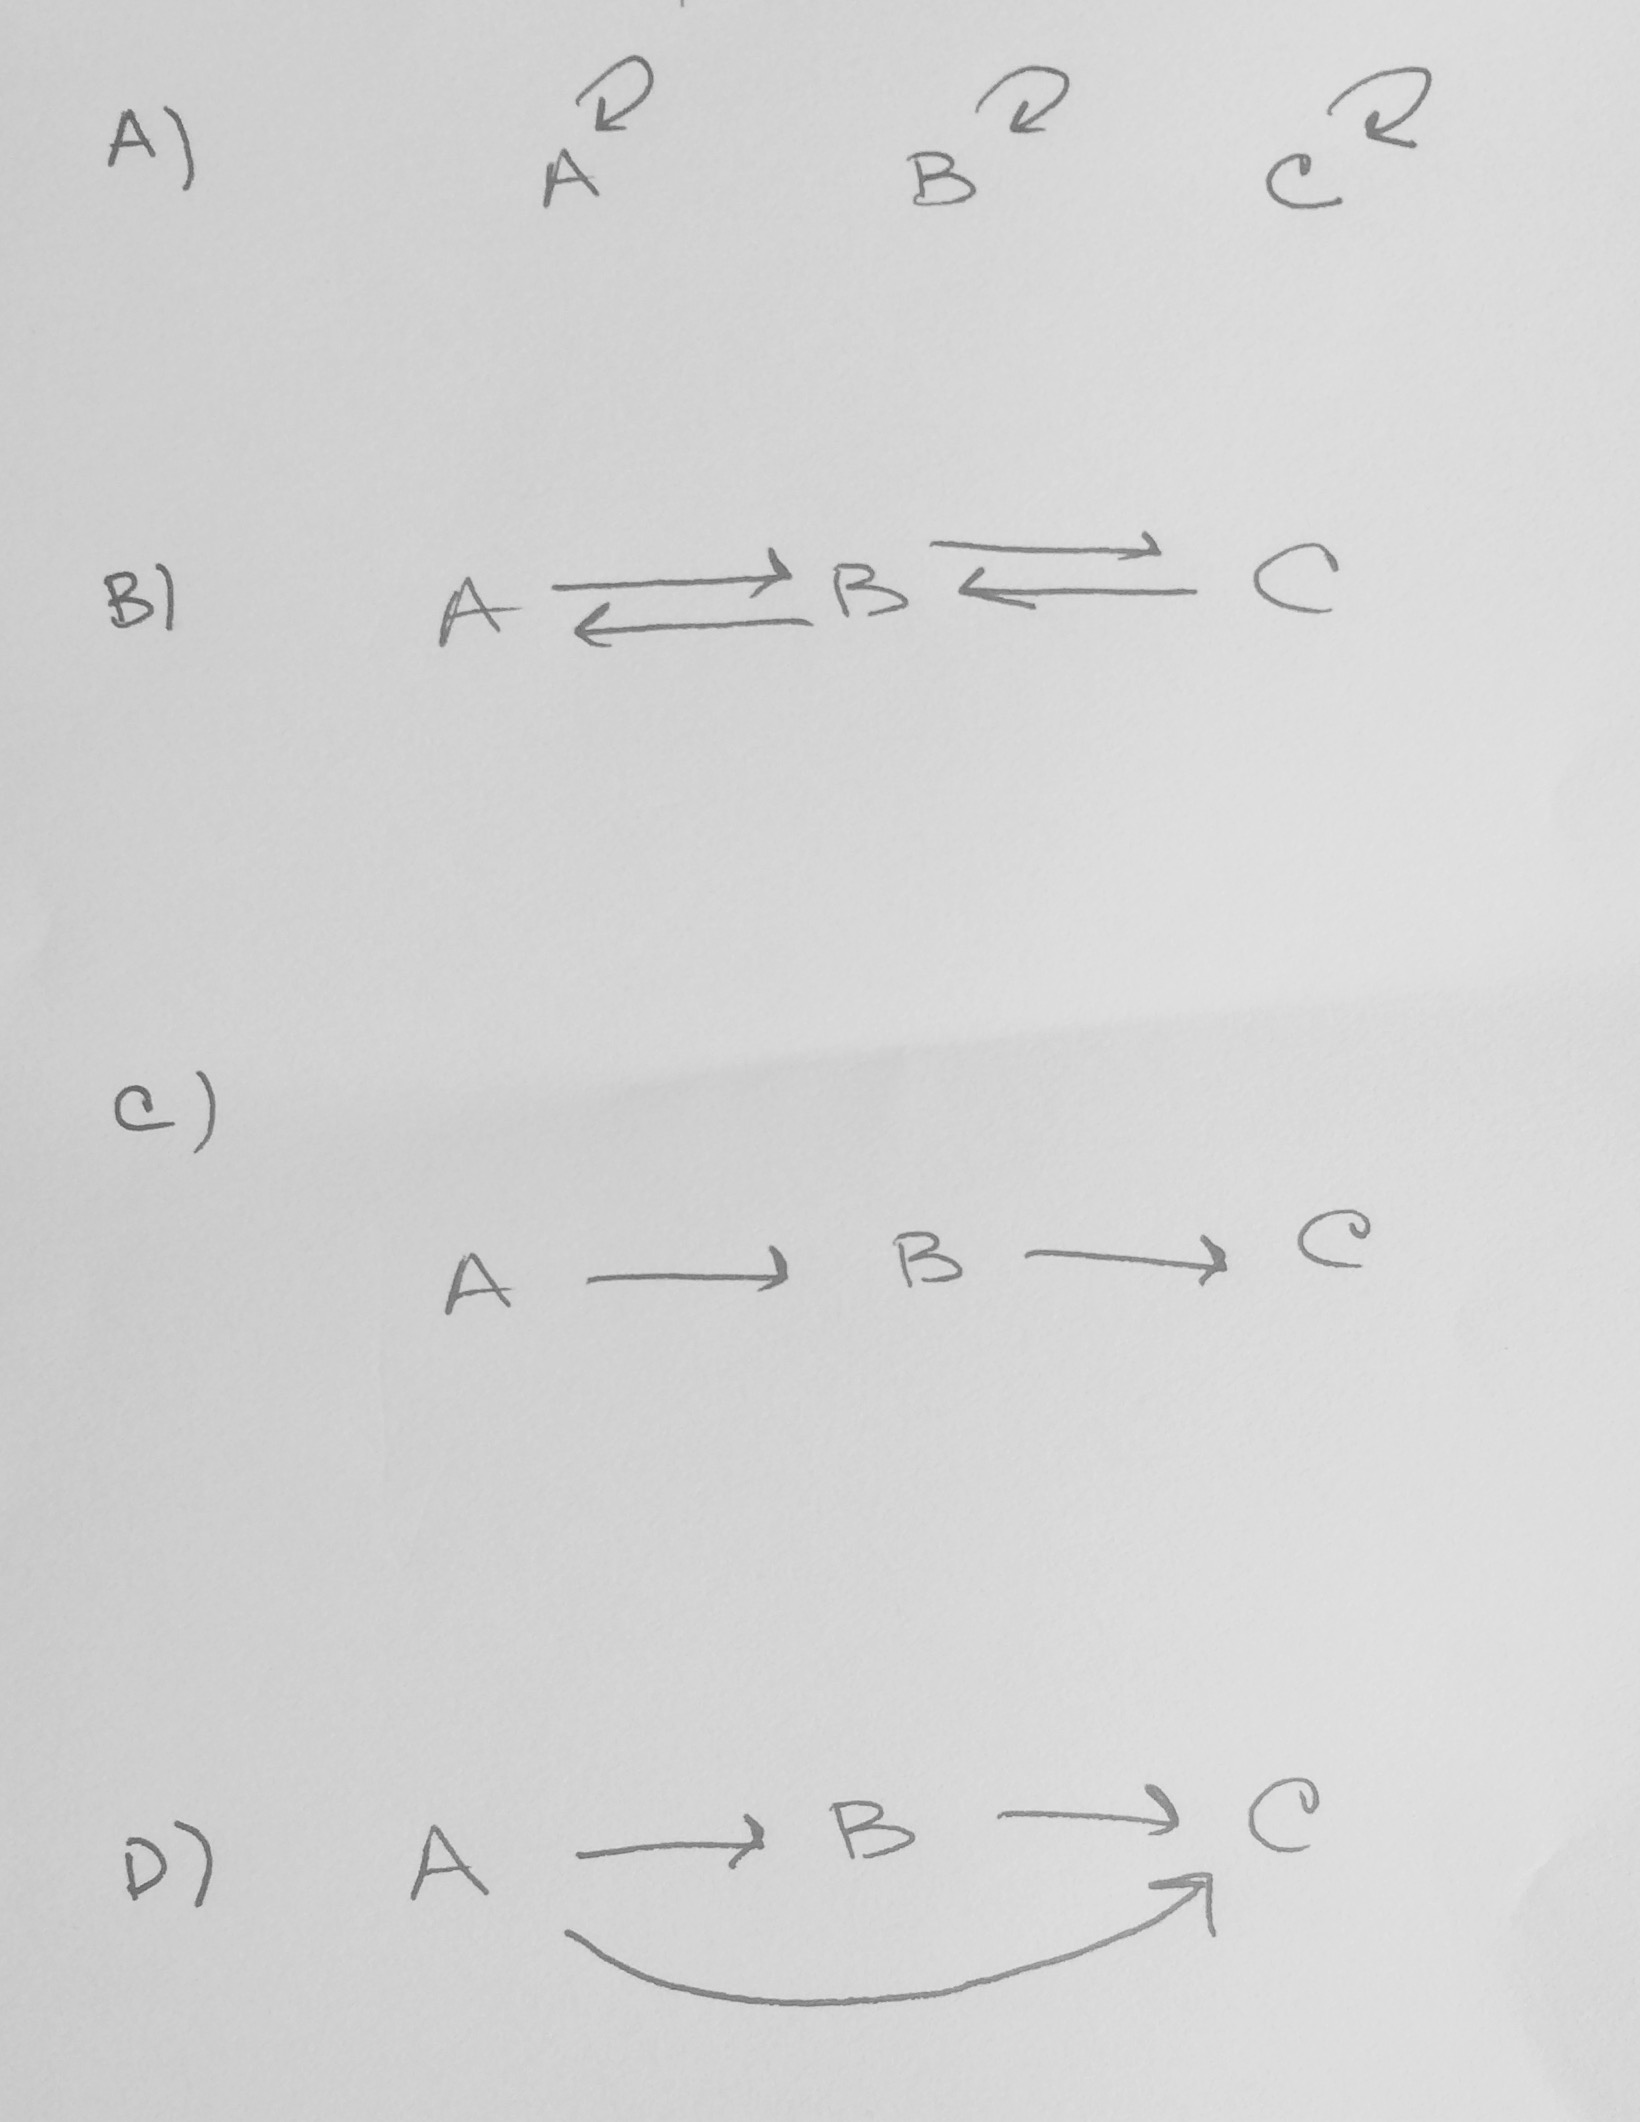
\includegraphics[width=3in]{3NodeGraphs.jpg}



\end{solution}

\problem

\subproblem Explain the difference between irreflexive and not reflexive
\subproblem Explain the difference between not symmetric, asymmetric, and antisymmetric. 
\subproblem Prove that if a relation $R$ is transitive and irreflexive, then it is asymmetric.

\begin{solution}
\subproblem Irreflexive is the negative of the universal (every possible relation is not reflexive). No node in an irreflexive graph has a self loop. Not reflexive means that there is at least one relation that is not reflexive. A graph that is not reflexive could have some self loops, but must have at least one node for which there is no self loop. 
\subproblem Asymmetric is the negative of the universal (every relation is not symmetric) where as a a relation is not symmetric if there were any instance where the relation is not symmetric. Antisymmetric is the same as asymmetric, except that an element may be in the relation with itself.
\subproblem Proof by contradiction. Assume for a moment the graph is not symmetric. Let us consider two connected nodes in the graph $a$ and  $b$. If there is an edge from $a$ to $b$  then there must also be edges from $b$ to $a$ since the graph is symmetric. Since the graph is transitive, there also be an edge from $a$ to $a$. However, we now have a contradiction since the graph is irreflexive. The graph must be asymmetric. 


\end{solution}

\problem Say that a string $x$ overlaps a string $y$ if there exist strings $p,q,r$ such that $x = pq$ and $y = qr$, with $q \neq \epsilon$. For example, $abcde$ overlaps $cdefg$, but does not overlap $bcd$ or $cdab$. Answer each of the following questions and prove your answer, or provide a counterexample. Consider the domain of all non-empty strings. 

\subproblem Is the overlap relation reflexive? 
\subproblem Is it symmetric?
\subproblem Is it transitive?

\begin{solution}
\subsolution Yes. A string will always overlap with itself, the entire string becomes the q section. 
\subsolution No. Counterexample: consider strings $abc$ and $bcx$. These strings overlap, but $bcx$ and $abc$ do not overlap. 
\subsolution No. Consider strings $abc$, $cde$, $efg$, $abc$ and $cde$ overlap, as do $cde$ and $efg$. However, $abc$ and $efg$ do not overlap. 

 
\end{solution}

\problem [BONUS] Determine what properties each of the following relations have. For those that are equivalence relations, briefly describe what the equivalence classes are in the relation.

\subproblem The relation ``shares a class with'', where two people share a class if there is a class they are both enrolled in this semester.
\subproblem The relation $R$ on $\mathbb{Z}$, where $aRb$ if $b$ is a multiple of $a$.


\begin{solution}
\subsolution Reflexive: you always share a class with yourself. Symmetric: if you are taking the same class as another person, then they are taking a class with you. NOT transitive. 
\subsolution Reflexive: a number always is a multiple of itself.  Transitive: consider $aRb$ and  $bRc$ $b = ax$, $c = by$. Thus, $c = axy$, where $xy$ is some multiplier. Not necessarily symmetric. 

\end{solution}




\end{document}
